\documentclass[linenumbers]{aastex631} %[twocolumn]

\newcommand{\vdag}{(v)^\dagger}
\newcommand\aastex{AAS\TeX}
\newcommand\latex{La\TeX}

\begin{document}

\title{Tracking Mass Transfer between M31 and the Milky Way using Galactic Simulation Data}


\author{Avichal Kaul}
\affiliation{Steward Observatory, University of Arizona, 933 N. Cherry Ave, Tucson, AZ 85721, USA}


\section{Introduction}

We wish to study the evolution of the Milky Way/M31 galactic merger. Specifically, the nature of the mass transfer during the merger, and the evolution of the entire system with time. 

Galactic Mergers are a process during which two or more galaxies, due to a combination of gravitational attraction and dynamic friction, fall together and merge into one galaxy. During this process, the star formation rate is increased hugely (\cite{Moster_2011}) and the structure of the galaxy undergoes massive changes - often, structures such as tidal tails are introduced, though these are not exclusive to galactic mergers. An example of one of these mergers can be seen in Figure \ref{fig:Privon image}.


Galactic mergers are an incredibly important aspect of galactic evolution. \cite{1978MNRAS.183..341W} notes that the $\lambda\text{CDM}$ model of cosmology suggests present day galaxies are formed from successive accretions and mergers of smaller entities. These successive accretions and mergers have been linked to star formation (\cite{Barnes_2004}) due to the sudden collision and compression of large HI clouds. Even the formation of tidal tails  are directly linked to the tidal forces exerted by other galaxies.

While the process of galaxies accreting and merging is well understood, there are still various open questions in this field. For instance, the role that supermassive black holes and Active Galactic Nuclei have to play during a merger.

\begin{figure}
    \centering
    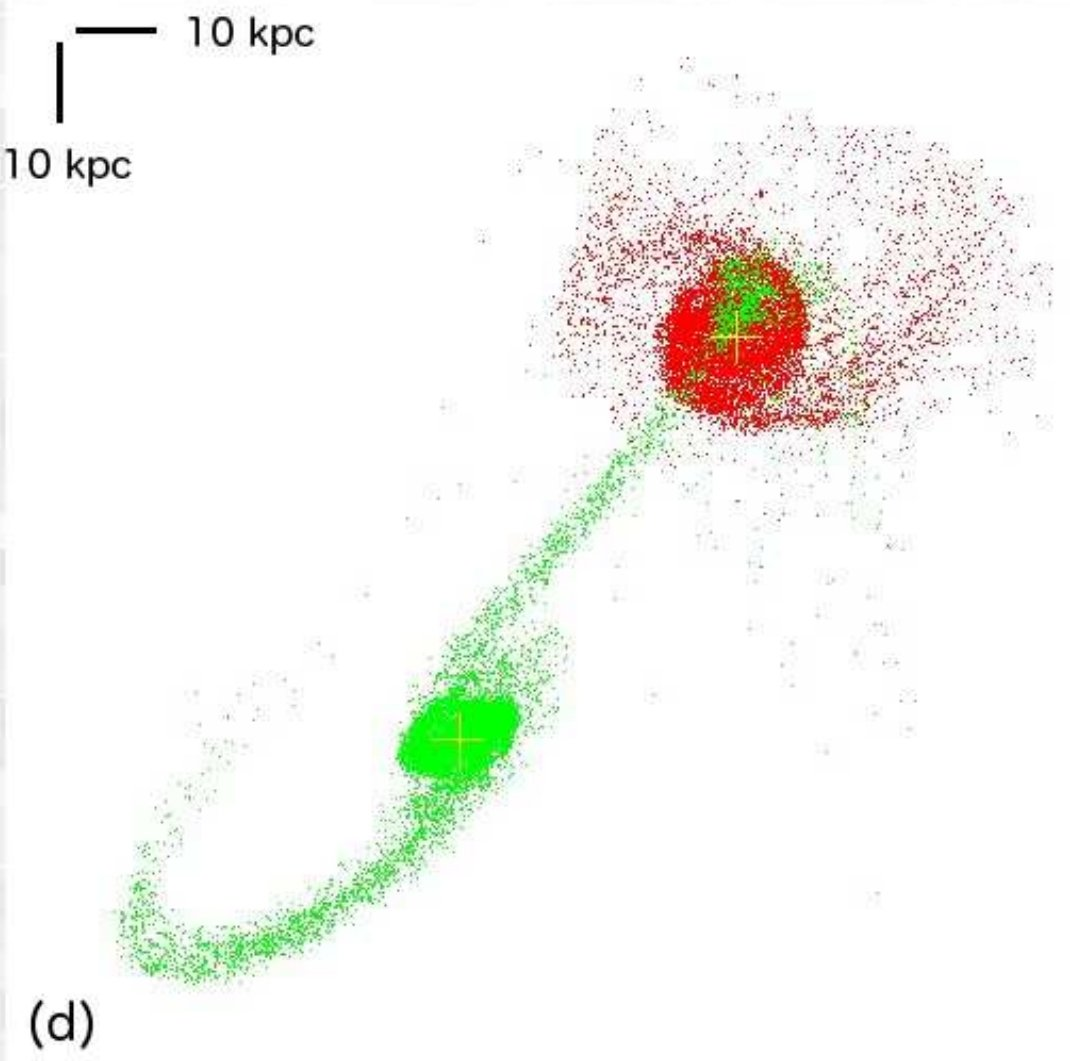
\includegraphics[width = 0.5\linewidth]{page08_1.jpg}
    \label{fig:Privon image}
    \caption{A snapshot from a galactic merger simulation that shows mass transfer between two galaxies. Figure from \cite{Privon_2013}.}
\end{figure}


\section{Proposal}

In the following sections, we will consider Galaxy A (stationary in its reference frame) and Galaxy B (colliding with Galaxy A). In actuality, both galaxies are moving towards each other. All the analysis described here will be performed on both the galaxies separately.

\subsection{Mass Transfer}

We can track the process of exchanging material by labelling the particles in the simulation with the name of their progenitor, then - after an encounter - checking to see if any particles have been exchanged between the galaxies. This only requires us to know the location of each particle, and the location of the galactic centre. For instance: we can use our previously developed code to find the location of Galaxy B's centre, and then check if any of the particles from Galaxy A have ended up there.

\subsection{Exchanged Material and its Kinematics}

To find which region of the galaxy the particles end up in, we can use a similar approach. As we know the position of the particles Galaxy A has exchanged with Galaxy B, we can check the main type of Galaxy B particle that surrounds them. Similarly, we can check if the particles rotate with the disk by calculating the velocity vector of Galaxy A's particles and comparing them to Galaxy B's particles. 

Finally, to track the total mass transfer over time, we can continue measuring how many particles have switched galaxies at regular timesteps until the galactic merger is complete.

\subsection{Evolution with Time}

I expect that, during the first couple of close encounters, most of the exchanged material will end up near the galactic centre. We can see this happening in simulation data (e.g. in Fig. \ref{fig:Privon image}). This makes sense, as the galactic centre is where most of the baryonic matter in the galaxy is concentrated. But, over time, the two galaxies will merge completely, so the material will all fall together into an elliptical galaxy.

\begin{figure}
    \centering
    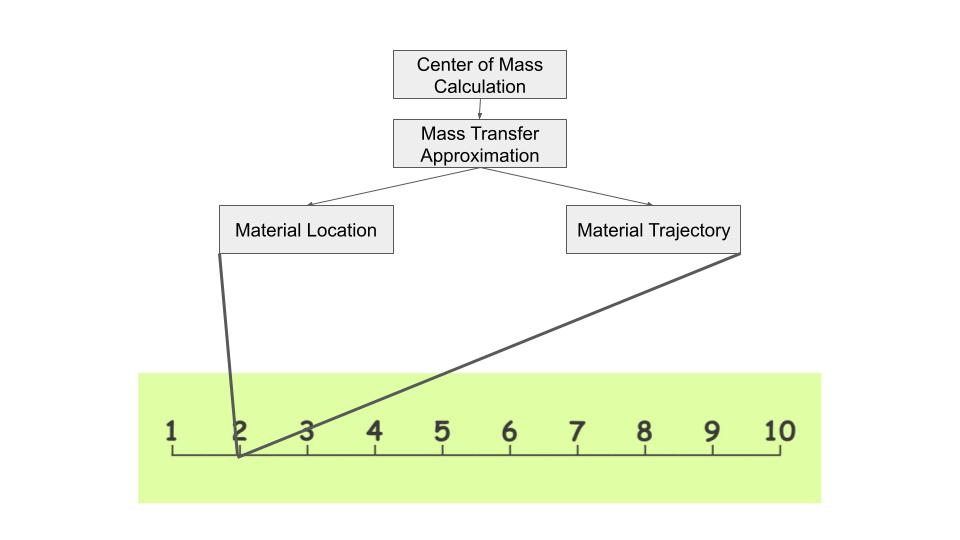
\includegraphics[width = \linewidth]{Untitled presentation.jpg}
    \label{fig:Untitled image}
    \caption{The proposed pipeline for data processing. At each simulation timestep (numbers 1-10 chosen for illustrative purposes), code is run to determine each property of the transferred material from top to bottom. This gives us an excellent idea of the evolution of the system with time.}
\end{figure}

\bibliography{sample631}{}
\bibliographystyle{aasjournal}

\end{document}